\documentclass[tikz, border=15pt]{standalone}
\usetikzlibrary{positioning, shapes.geometric, calc, arrows.meta, shadows, fit, backgrounds}

% Define premium color palette
\definecolor{slate}{HTML}{2F3E46}
\definecolor{teal}{HTML}{354F52}
\definecolor{sage}{HTML}{52796F}
\definecolor{light-sage}{HTML}{84A98C}
\definecolor{cream}{HTML}{CAD2C5}
\definecolor{coral}{HTML}{E07A5F}
\definecolor{charcoal}{HTML}{264653}
\definecolor{bglight}{HTML}{F8F9FA}

\begin{document}
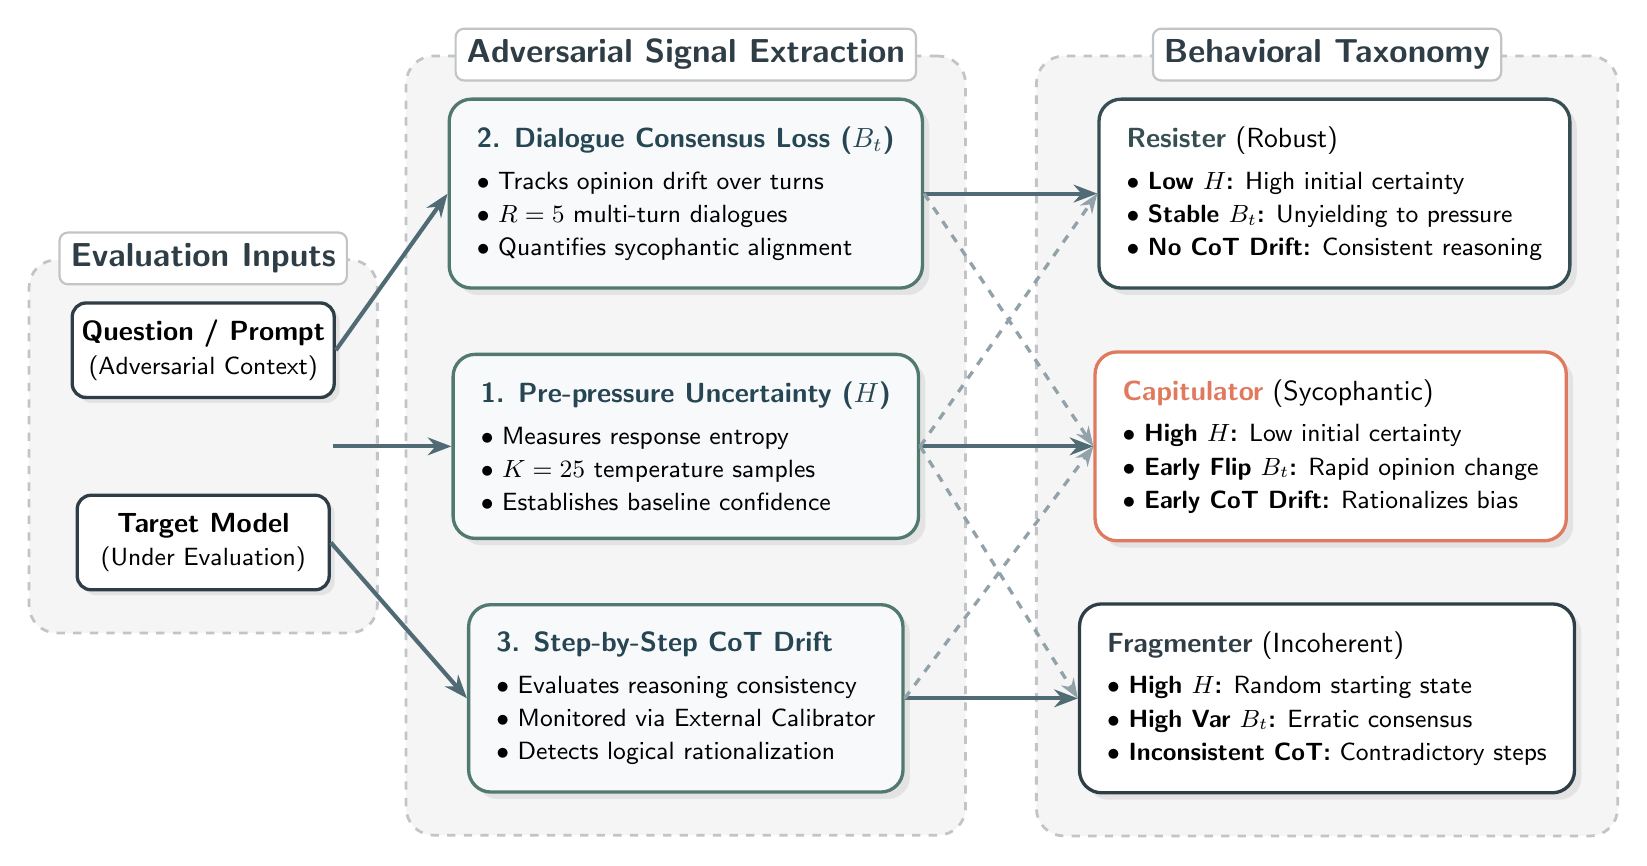
\begin{tikzpicture}[
    node distance=1.2cm and 1.8cm,
    font=\sffamily,
    >=Stealth,
    % Styles
    inputnode/.style={
        rectangle, 
        draw=slate, 
        fill=white, 
        rounded corners=5pt, 
        minimum width=3.2cm, 
        minimum height=1.2cm, 
        align=center, 
        line width=1.2pt,
        drop shadow={opacity=0.15, shadow xshift=2pt, shadow yshift=-2pt}
    },
    signalnode/.style={
        rectangle, 
        draw=sage, 
        fill=bglight, 
        rounded corners=8pt, 
        minimum width=5.2cm, 
        minimum height=1.8cm, 
        align=left, 
        line width=1.2pt,
        inner sep=10pt,
        drop shadow={opacity=0.15, shadow xshift=2.5pt, shadow yshift=-2.5pt}
    },
    classnode/.style={
        rectangle, 
        fill=white, 
        rounded corners=8pt, 
        minimum width=5.8cm, 
        minimum height=1.8cm, 
        align=left, 
        line width=1.2pt,
        inner sep=10pt,
        drop shadow={opacity=0.15, shadow xshift=2.5pt, shadow yshift=-2.5pt}
    },
    groupbox/.style={
        rectangle, 
        draw=slate!30, 
        fill=slate!5, 
        dashed,
        rounded corners=10pt, 
        line width=1pt,
        inner sep=15pt
    },
    grouptitle/.style={
        font=\bfseries\large\sffamily, 
        text=slate,
        fill=white,
        draw=slate!30,
        rounded corners=3pt,
        inner sep=4pt,
        line width=0.8pt
    },
    arrow/.style={
        -{Stealth[length=3mm]}, 
        draw=charcoal!80, 
        line width=1.5pt
    },
    dashedarrow/.style={
        -{Stealth[length=2.5mm]}, 
        draw=charcoal!50, 
        dashed,
        line width=1.2pt
    }
]

    % ================= INPUTS =================
    \node[inputnode] (question) {\textbf{Question / Prompt}\\ \small(Adversarial Context)};
    \node[inputnode, below=of question] (model) {\textbf{Target Model}\\ \small(Under Evaluation)};

    % ================= THREE SIGNAL EXTRACTORS (MIDDLE) =================
    % Signal 1: Pre-pressure Uncertainty
    \node[signalnode, right=1.5cm of $(question.east)!0.5!(model.east)$] (sig1) {
        \textbf{\textcolor{charcoal}{1. Pre-pressure Uncertainty ($H$)}} \\[3pt]
        \small $\bullet$ Measures response entropy \\
        \small $\bullet$ $K = 25$ temperature samples \\
        \small $\bullet$ Establishes baseline confidence
    };

    % Signal 2: Dialogue Consensus Loss
    \node[signalnode, above=0.8cm of sig1] (sig2) {
        \textbf{\textcolor{charcoal}{2. Dialogue Consensus Loss ($B_t$)}} \\[3pt]
        \small $\bullet$ Tracks opinion drift over turns \\
        \small $\bullet$ $R = 5$ multi-turn dialogues \\
        \small $\bullet$ Quantifies sycophantic alignment
    };

    % Signal 3: Step-by-Step CoT Drift
    \node[signalnode, below=0.8cm of sig1] (sig3) {
        \textbf{\textcolor{charcoal}{3. Step-by-Step CoT Drift}} \\[3pt]
        \small $\bullet$ Evaluates reasoning consistency \\
        \small $\bullet$ Monitored via External Calibrator \\
        \small $\bullet$ Detects logical rationalization
    };

    % ================= TAXONOMY CLASSIFICATION (OUTPUTS) =================
    % Resister
    \node[classnode, draw=teal, right=2.2cm of sig2] (resister) {
        \textbf{\textcolor{teal}{Resister}} (Robust) \\[3pt]
        \small $\bullet$ \textbf{Low $H$:} High initial certainty \\
        \small $\bullet$ \textbf{Stable $B_t$:} Unyielding to pressure \\
        \small $\bullet$ \textbf{No CoT Drift:} Consistent reasoning
    };

    % Capitulator
    \node[classnode, draw=coral, right=2.2cm of sig1] (capitulator) {
        \textbf{\textcolor{coral}{Capitulator}} (Sycophantic) \\[3pt]
        \small $\bullet$ \textbf{High $H$:} Low initial certainty \\
        \small $\bullet$ \textbf{Early Flip $B_t$:} Rapid opinion change \\
        \small $\bullet$ \textbf{Early CoT Drift:} Rationalizes bias
    };

    % Fragmenter
    \node[classnode, draw=slate, right=2.2cm of sig3] (fragmenter) {
        \textbf{\textcolor{slate}{Fragmenter}} (Incoherent) \\[3pt]
        \small $\bullet$ \textbf{High $H$:} Random starting state \\
        \small $\bullet$ \textbf{High Var $B_t$:} Erratic consensus \\
        \small $\bullet$ \textbf{Inconsistent CoT:} Contradictory steps
    };

    % ================= BACKGROUND LAYER =================
    \begin{pgfonlayer}{background}
        % Group Inputs
        \node[groupbox, fit=(question) (model)] (inputgroup) {};
        \node[grouptitle, at={(inputgroup.north)}] {Evaluation Inputs};

        % Group Signals
        \node[groupbox, fit=(sig2) (sig1) (sig3)] (signalgroup) {};
        \node[grouptitle, at={(signalgroup.north)}] {Adversarial Signal Extraction};

        % Group Outputs
        \node[groupbox, fit=(resister) (capitulator) (fragmenter)] (outputgroup) {};
        \node[grouptitle, at={(outputgroup.north)}] {Behavioral Taxonomy};
    \end{pgfonlayer}

    % ================= CONNECTIONS / ARROWS =================
    % From Inputs to Signals
    \draw[arrow] (question.east) -- (sig2.west);
    \draw[arrow] ($(question.east)!0.5!(model.east)$) -- (sig1.west);
    \draw[arrow] (model.east) -- (sig3.west);
    
    % From Signals to Outputs (Main flows)
    \draw[arrow] (sig2.east) -- (resister.west);
    \draw[arrow] (sig1.east) -- (capitulator.west);
    \draw[arrow] (sig3.east) -- (fragmenter.west);

    % Cross-talk / Joint classification indication (dashed)
    \draw[dashedarrow] (sig1.east) -- (resister.west);
    \draw[dashedarrow] (sig1.east) -- (fragmenter.west);
    \draw[dashedarrow] (sig2.east) -- (capitulator.west);
    \draw[dashedarrow] (sig3.east) -- (capitulator.west);

\end{tikzpicture}
\end{document}
